\begin{figure}[htb!]
	\centering
	\footnotesize

	\psfrag{a}[c][c] {$5$}
	\psfrag{b}[c][c] {$1$}
	\psfrag{c}[c][c] {$2$}

	\psfrag{d}[c][c] {$0$}
	\psfrag{e}[c][c] {$-1$}
	\psfrag{f}[c][c] {$0$}

	\psfrag{g}[c][c] {$0$}
	\psfrag{h}[c][c] {$1$}
	\psfrag{i}[c][c] {$6$}

	\psfrag{n}[c][c] {$0$}

	\psfrag{A}[c][c] {$A=$}
	\psfrag{P}[c][c] {$P_{1}A=$}
	\psfrag{Q}[c][c] {$P_{2}P_{1}A=$}
	\psfrag{M}[c][c] {$P_{3}P_{2}P_{1}A=$}


	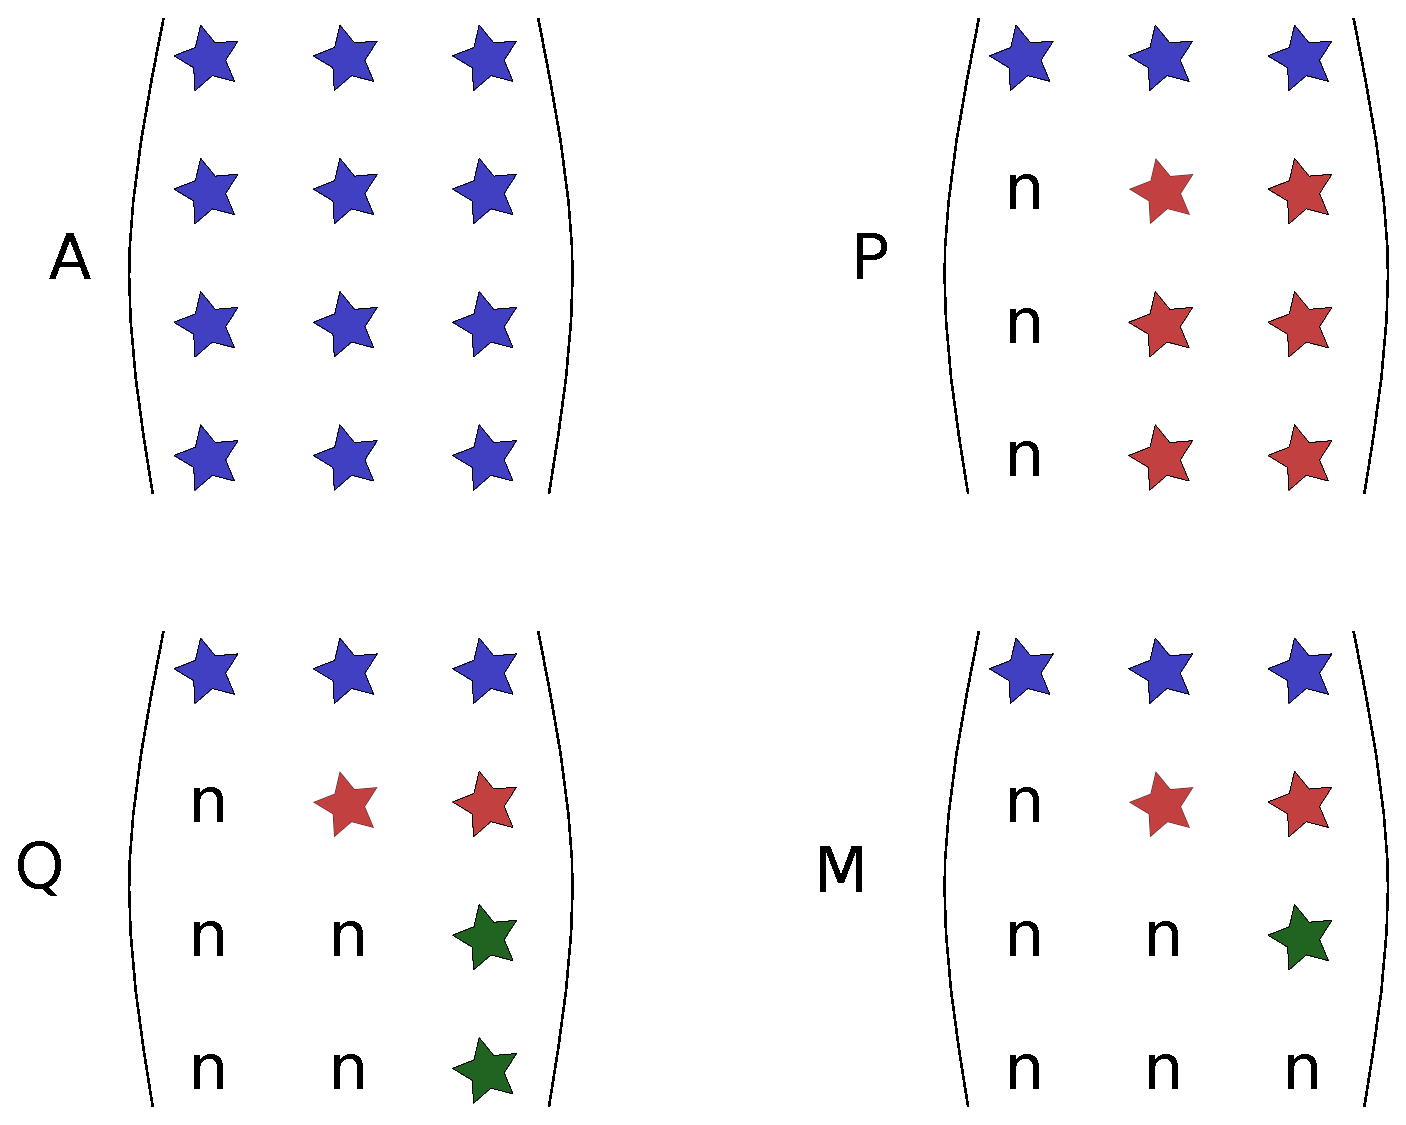
\includegraphics[width=0.99\textwidth]{householder.eps}
	\caption{How Householder-Reflection actually works: Given matrix $A$.
	We would like to apply a matrix $P_1$ on the left side of matrix $A$ 
	in such a way that the resulting matrix has the first row unchanged, 
	and any first entry from the second row onwards turn to zero. 
	This procedure is repeated until the final resulting matrix becomes
	a right upper triangular matrix.}
	\label{\LABEL}
\end{figure}
